\section{PyLith Output}

PyLith currently supports output to VTK and HDF5/Xdmf files, which
can be imported directly into a number of visualization tools, such
as ParaView, Visit, and MayaVi. The HDF5 files can also be directly
accessed via Matlab and PyTables. PyLith v1.1 significantly expanded
the information available for output, including fault information
and state variables. Output of solution information for the domain,
faults, materials, and boundary conditions is controlled by an output
manager for each module. This allows the user to tailor the output
to the problem. By default PyLith will write a number of files. Diagnostic
information for each fault and material is written into a separate
file as are the solution and state variables for the domain, each
fault, and each material. For a fault the diagnostic fields include
the final slip, the slip initiation time, and the fault normal vector.
For a material the diagnostic fields include the density and the elastic
constants. Additional diagnostic information can be included by setting
the appropriate output parameters. See Chapters \vref{cha:material:models}
and \vref{cha:boundary:interface:conditions} for more information
on the available fields and the next section for output parameters.
The other files for each fault and material include solution information
at each time step where output was requested (also customizable by
the user). For a fault the solution information includes the slip
and the change in tractions on the fault surface. For a material the
solution information includes the total strain and stress. For some
materials fields for additional state variables may be available.
For output via VTK files, each time step is written to a separate
file, whereas for HDF5 files all of the time steps for a given domain,
fault, or material are written into the same file. A single Xdmf metadata
file is created for each HDF5 file.


\subsection{Output Manager}

The \object{OutputManager} object controls the type of files written, the fields
included in the output, and how often output is written. PyLith includes
some specialized OutputManagers that prescribe what fields are output
by default. In some cases, additional fields are available but not
included by default. For example, in 3D problems, the along-strike
and up-dip directions over the fault surface can be included in the
diagnostic information. These are not included by default, because
1D problems have neither an along-strike nor up-dip direction and
2D problems do not have an up-dip direction.


The parameters for the \object{OutputManager} are:
\begin{inventory}
\propertyitem{output\_freq}{Flag indicating whether to write output based on
the time or number of time steps since the last output. Permissible
values are ``time\_step'' and ``skip'' (default).}
\propertyitem{time\_step}{Minimum time between output if \property{output\_freq}
is set to ``time\_step''.}
\propertyitem{skip}{Number of time steps between output if \property{output\_freq}
is set to ``skip''. A value of 0 means every time step is written.}
\facilityitem{writer}{Writer for data (VTK writer or HDF5 writer).}
\facilityitem{coordsys}{Coordinate system for vertex coordinates (currently
ignored).}
\facilityitem{vertex\_filter}{Filter to apply to all vertex fields (see Section
\vref{sub:vertex:field:filters}).}
\facilityitem{cell\_filter}{Filter to apply to all cell fields (see Section
\vref{sub:cell:field:filters}).}
\end{inventory}
An example of setting the output parameters for a material in a \filename{.cfg}
file is
\begin{cfg}
<h>[pylithapp.timedependent.materials.elastic.output]</h>
<p>output_freq</p> = time_step
<p>time_step</p> = 1.0*yr
<f>cell_filter</f> = pylith.meshio.CellFilterAvg
<p>cell_info_fields</p> = [density] ; limit diagnostic data to density
<p>cell_data_fields</p> = [total-strain, stress] ; default
<p>writer.filename</p> = dislocation-elastic.vtk
\end{cfg}

\subsubsection{Output Over Subdomain}
\label{sec:output:subdomain}

Output of the solution over the entire domain for large problems generates
very large data files. In some cases one is primarily interested in
the solution over the ground surface. PyLith supports output of the
solution on any boundary of the domain by associating an output manager
with a group of vertices corresponding to the surface of the boundary.
As with several of the boundary conditions, the boundary must be a
simply-connected surface. The \object{OutputSolnSubset} is the specialized
\object{OutputManager} that implements this feature and, by default, includes
the displacement field in the output. In addition to the \object{OutputManager}
parameters, the \object{OutputSolnSubset} includes:
\begin{inventory}
\propertyitem{label}{Label of group of vertices defining boundary surface.}
\propertyitem{vertex\_data\_fields}{Names of vertex data fields to output (default
is [displacement]).}
\end{inventory}

\subsection{Output at Arbitrary Points}
\label{sec:output:points}

In many situations with recorded observations, one would like to
extract the solution at the same locations as the recorded
observation. Rather than forcing the finite-element discretization to
be consistent with the observation points, PyLith includes a
specialized output manager, \object{OutputSolnPoints}, to interpolate
the solution to arbitrary points. By default, the output manager will
include the displaceent time histories in the output. The locations
are specified in a text file. In addition to the
\object{OutputManager} parameters, the \object{OutputSolnSubset}
includes:
\begin{inventory}
\propertyitem{vertex\_data\_fields}{Names of vertex data fields to output (default
is [displacement]).}
\facilityitem{reader}{Reader for points list (default is \object{PointsList}).}
\facilityitem{writer}{Writer for output (default is \object{DataWriterVTKPoints}). In most cases users will want to use the \object{DataWriterHDF5}.}
\end{inventory}

\subsubsection{\object{PointsList} Reader}

This object corresponds to a simple text file containing a list of
points (one per line) where output is desired. See \vref{sec:format:PointsList}
for file format specifications. The points are specified in the coordinate
system specified by \object{OutputSolnPoints}. The coordinates will be transformed
into the coordinate system of the mesh prior to interpolation. The
properties available to customize the behavior of \object{PointsList}
are:
\begin{inventory}
\propertyitem{filename}{Names of file containing list of points.}
\propertyitem{comment\_delimiter}{Delimiter at beginning of line to identify
comments (default is \#).}
\propertyitem{value\_delimiter}{Delimiter used to separate values (default is
whitespace).}
\end{inventory}

\subsection{Output Field Filters}

Output fields may not directly correspond to the information a user
desires. For example, the default output for the state variables
includes the values at each quadrature point. Most visualization
packages cannot handle cell fields with multiple points in a cell (the
locations of the points within the cell are not included in the data
file). In order to reduce the field to a single point within the cell,
we would like to average the values. This is best done within PyLith
before output, because it reduces the file size and the quadrature
information provides the information necessary (the weights of the
quadrature points) to compute the appropriate average over the cell.

\subsubsection{Vertex Field Filters}
\label{sub:vertex:field:filters}

Currently the only filter available for vertex fields computes the
magnitude of a vector at each location. Most visualization packages
support this operation, so this filter is not used very often.
\begin{description}
\item [\object{VertexFilterVecNorm}] Computes the magnitude of a vector field
at each location.
\end{description}

\subsubsection{Cell Field Filters}
\label{sub:cell:field:filters}

Most users will want to apply a filter to cell fields to average the
fields over the cell, producing values at one location per cell for
visualization.
\begin{description}
\item [\object{CellFilterAvg}] Compute the weighted average of the values within
a cell. The weights are determined from the quadrature associated
with the cells.
\end{description}

\subsection{VTK Output (\object{DataWriterVTK})}

PyLith writes legacy (non-XML) VTK files. These are simple files with
vertex coordinates, the mesh topology, and fields over vertices and/or
cells. Each time step is written to a different file. The time stamp
is included in the filename with the decimal point removed. This allows
automatic generation of animations with many visualization packages
that use VTK files. The default time stamp is the time in seconds,
but this can be changed using the normalization constant to give a
time stamp in years, tens of years, or any other value.


The parameters for the VTK writer are:
\begin{inventory}
\propertyitem{filename}{Name of VTK file.}
\propertyitem{time\_format}{C-style format string for time stamp in filename.
The decimal point in the time stamp will be removed for compatibility
with VTK visualization packages that provide seamless animation of
data from multiple VTK files.}
\propertyitem{time\_constant}{Value used to normalize time stamp in VTK files
(default is 1.0 s).}
\end{inventory}

\subsection{HDF5/Xdmf Output (\object{DataWriterHDF5}, \object{DataWriterHDF5Ext})}
\label{sub:HDF5/Xdmf-Output}

HDF5 files provide a flexible framework for storing simulation data
with datasets in groups logically organized in a tree structure analogous
to files in directories. HDF5 output offers parallel, multi-dimensional
array output in binary files, so it is much faster and more convenient
than the VTK output which uses ASCII files and separate files for
each time step. Standards for organizing datasets and groups in HDF5
files do not exist for general finite-element software in geodynamics.
Consequently, PyLith uses its own simple layout show in Figure \vref{fig:hdf5:layout}.
In order for visualization tools, such as ParaView, to determine which
datasets to read and where to find them in the hierarchy of groups
within the HDF5 file, we create an Xdmf (eXtensible Data Model and
Format, \url{www.xdmf.org}) metadata file that provides this information.
This file is written when PyLith closes the HDF5 file at the end of
the simulation. In order to visualize the datasets in an HDF5 file,
one simply opens the corresponding Xdmf file (the extension is \filename{.xmf})
in ParaView or Visit. The Xdmf file contains the relative path to
the HDF5 file so the files can be moved but must be located together
in the same directory. 

\important{The Xdmf format supports
representation of two- and three-dimensional coordinates of points,
scalar fields, and three-dimensional vector and tensor fields but
not two-dimensional vector or tensor fields. Consequently, for two-dimensional
vector fields we build a three-component vector from the two-component
vector (x and y components) and a separate zero scalar field (z component).
For tensor fields, we create a scalar field for each of the tensor
components, adding the component as a suffix to the name of the field.}

\begin{figure}[htbp]
  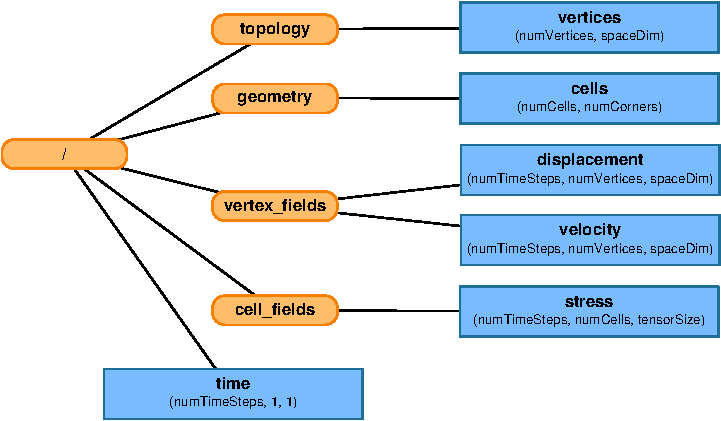
\includegraphics{runpylith/figs/hdf5layout}
  \caption{General layout of a PyLith HDF5 file. The orange rectangles
    with rounded corners identify the groups and the blue rectangles
    with sharp corners identify the datasets. The dimensions of the
    data sets are shown in parentheses. Most HDF5 files will contain
    either \texttt{vertex\_fields} or \texttt{cell\_fields} but not
    both.}
 \label{fig:hdf5:layout}
\end{figure}

See Table \vref{tab:materials:statevars} in Section
\vref{sec:material:parameters} for a table of component values for
tensor output in HDF5 files. To avoid confusion about the ordering of
components for tensor data, we separate the components in the Xdmf
file.

HDF5 files do not contain self-correcting features that allow a file
to be read if part of a dataset is corrupted. This type of error can
occur if a job terminates abnormally in the middle or at the end of a
simulation on a large cluster or other parallel machine. Fortunately,
HDF5 also offers the ability to store datasets in external binary
files with the locations specified by links in the HDF5 file. Note
that the use of external data files results in one data file per
dataset in addition to the HDF5 and Xdmf files. The external data
files use the name of the HDF5 file with the dataset name added to the
prefix and the \filename{.h5} suffix replaced by \filename{.dat}. The
HDF5 files include relative paths to the external data files, so these
files can also be moved, but they, too, must be kept together in the
same directory. This provides a more robust method of output because
one can generate an HDF5 file associated with the uncorrupted portions
of the external data files should an error occur. Currently, PyLith
does not include a utility to do this, but we plan to add one in a
future release. Thus, there are two options when writing PyLith output
to HDF5 files: (1) including the datasets directly in the HDF5 files
themselves using the \object{DataWriterHDF5} object or (2) storing the
datasets in external binary files with just metadata in the HDF5 files
using the \object{DataWriterHDF5Ext} object. Both methods provide
similar performance because they will use MPI I/O if it is available.

\warning{Storing the datasets within the HDF5 file in a parallel
  simulation requires that the HDF5 library be configured with the
  \commandline{-{}-enable-parallel} option. The binary PyLith packages
  include this feature and it is a default setting in building HDF5
  via the PyLith Installer.}

Accessing the datasets for additional analysis or visualization is
nearly identical in the two methods because the use of external data
files is completely transparent to the user except for the presence
of the additional files. Note that in order for ParaView to find the
HDF5 and external data files, it must be run from the same relative
location where the simulation was run. For example, if the simulation
was run from a directory called ``work'' and the HDF5/Xdmf files
were written to ``work/output'', then ParaView should be run from
the ``work'' directory. See Table \vref{tab:materials:statevars}
in Section \vref{sec:material:parameters} for a table of component
values for tensor output.

\subsubsection{Parameters}

The parametesr for the \object{DataWriterHDF5} and
\object{DataWriterHDF5Ext} objects is identical:
\begin{inventory}
\propertyitem{filename}{Name of HDF5 file (the Xdmf filename is generated from
the same prefix).}
\end{inventory}

An example of changing the writer from the default VTK writer to the
HDF5 writer with external datasets (\object{DataWriterHDF5Ext}) for
output over the domain in a \filename{.cfg} file is
\begin{cfg}
<h>[pylithapp.timedependent.domain.output]</h>
<p>output_freq</p> = time_step
<p>time_step</p> = 1.0*yr
<p>cell_data_fields</p> = [displacement, velocity]
<f>writer</f> = pylith.meshio.DataWriterHDF5Ext
<p>writer.filename</p> = dislocation.h5
\end{cfg}


\subsubsection{HDF5 Utilities}

HDF5 includes several utilities for examining the contents of HDF5
files. \filename{h5dump} is very handy for dumping the hierarchy,
dimensions of datasets, attributes, and even the dataset values to
stdout. 
\begin{shell}
# Dump the entire HDF5 file (not useful for large files).
$$ h5dump mydata.h5
# Dump the hierarchy of an HDF5 file.
$$ h5dump -n mydata.h5
# Dump the hierarchy with dataset dimensions and attributes.
$$ h5dump -H mydata.h5
# Dump dataset 'vertices' in group '/geometry' to stdout.
$$ h5dump -d /geometry/vertices mydata.h5
\end{shell}
We have also include a utility \filename{pylith\_genxdmf} (see Section
\vref{sec:pylith:genxdmf}) that generates an appropriate Xdmf file
from a PyLith HDF5 file. This is very useful if you add fields to
HDF5 files in post-processing and wish to view the results in ParaView
or Visit.


% End of file
